\documentclass[12pt]{../manual}
%____________________________________________________________________________
%
%	TITLE AND TABLE OF CONTENTS
%____________________________________________________________________________
\begin{document}
\makeheader{Lab 6}
\begin{center}
\textbf{\huge ECE 230L - LAB 6}\\~\\
\textbf{\large MOSFET SIMULATION WITH PSPICE}\\~\\
\rule{6.5in}{0.5mm}\\
\end{center}

\tableofcontents

\listoffigures

\newpage
%____________________________________________________________________________
%
%	BODY
%____________________________________________________________________________
\section{Objectives of this Laboratory}
The objectives of this laboratory session are as follows:
\begin{itemize}
\item  Simulate an NMOSFET in PSpice
\item Use manufacturer, measured, and empirical average NMOSFET model parameters to evaluate
the transistor in PSpice
\item Compare the measured threshold voltage, transconductance, and channel-length modulation
parameters to those specified by the manufacturer
\end{itemize}

\section{PSpice simulation of a MOSFET}
The circuit used in the electrical characterization of the MOSFET is shown in Figure \ref{fig:nmosfet}. Using PSpice, simulate the drain current-voltage characteristics of the BS170 Metal-Oxide Semiconductor Field-Effect Transistor (MOSFET). The PSpice code to simulate and plot the $I_D (V_{GS}, V_{DS})$ drain-current characteristics of this N-channel MOSFET is given below. Use this model to create a PSpice input file for simulating the MOSFET characteristics. Note in particular the model parameters used for the threshold voltage ({\tt VTO}), the transconductance ({\tt KP}), and the channel-length modulation parameter ({\tt lambda}).

\begin{figure}[ht!]
\begin{center}
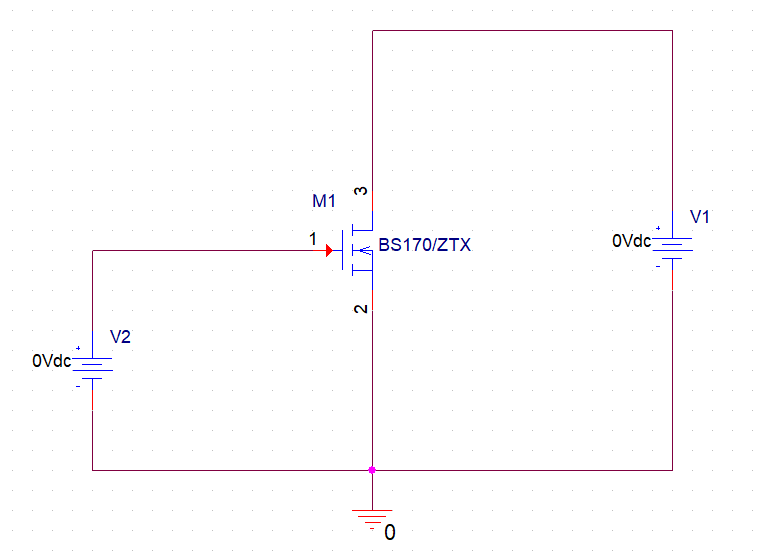
\includegraphics[width=0.8\textwidth]{figures/characterizeNMOS}
\end{center}
\caption{Circuit used to characterize an NMOSFET}
\label{fig:nmosfet}
\end{figure}

\newpage
\subsection{Placing an NMOS Transistor}
To add a transistor to your schematic select \textbf{Place} in your toolbar and then select \textbf{Part}. Use the `Add Library' button shown in Figure \ref{fig:placemenu} to search the \textbf{Library} $\to$ \textbf{PSpice} folder for the `ZETEX’ library.

\begin{figure}[ht!]
\begin{center}
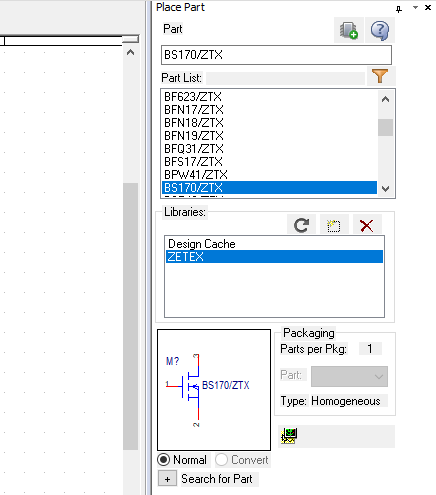
\includegraphics[width=0.6\textwidth]{figures/placeMenu}
\end{center}
\caption{Place part menu}
\label{fig:placemenu}
\end{figure}

Once you add the `ZETEX’ library, search for BS170/ZTX. Add this part to your schematic. You will need to add voltage sources to your schematic to represent $V_{GS}$ and $V_{DS}$ and wire them to match the circuit in Figure \ref{fig:nmosfet}.

\newpage
\subsection{Setting up the Simulation Profile}
\label{sim}
Use the following parameters to simulate the ZETEX BS170/ZTX MOSFET:
\begin{itemize}
\item Analysis Type: DC Sweep
\item Primary Sweep
\begin{itemize}
\item Voltage Source: $V_{DS}$ ($V_1$ in Figure \ref{fig:nmosfet}) 
\item Sweep Type: Linear
\item Start Value: \SI{0}{\volt}
\item End Value: \SI{5}{\volt}
\item Increment: \SI{0.01}{\volt} 
\end{itemize}
\item Secondary Sweep
\begin{itemize}
\item Voltage Source: $V_{GS}$ ($V_2$ in Figure \ref{fig:nmosfet}) 
\item Sweep Type: Linear
\item Start Value: \SI{2}{\volt}
\item End Value: \SI{3}{\volt}
\item Increment: \SI{0.25}{\volt}
\end{itemize}
\end{itemize}


Run your simulation and save your results. Use I(M1:D) as your trace. The results of the ZETEX BS170/ZTX simulation are shown in Figure \ref{fig:zetexsim}.

\begin{figure}[ht!]
\begin{center}
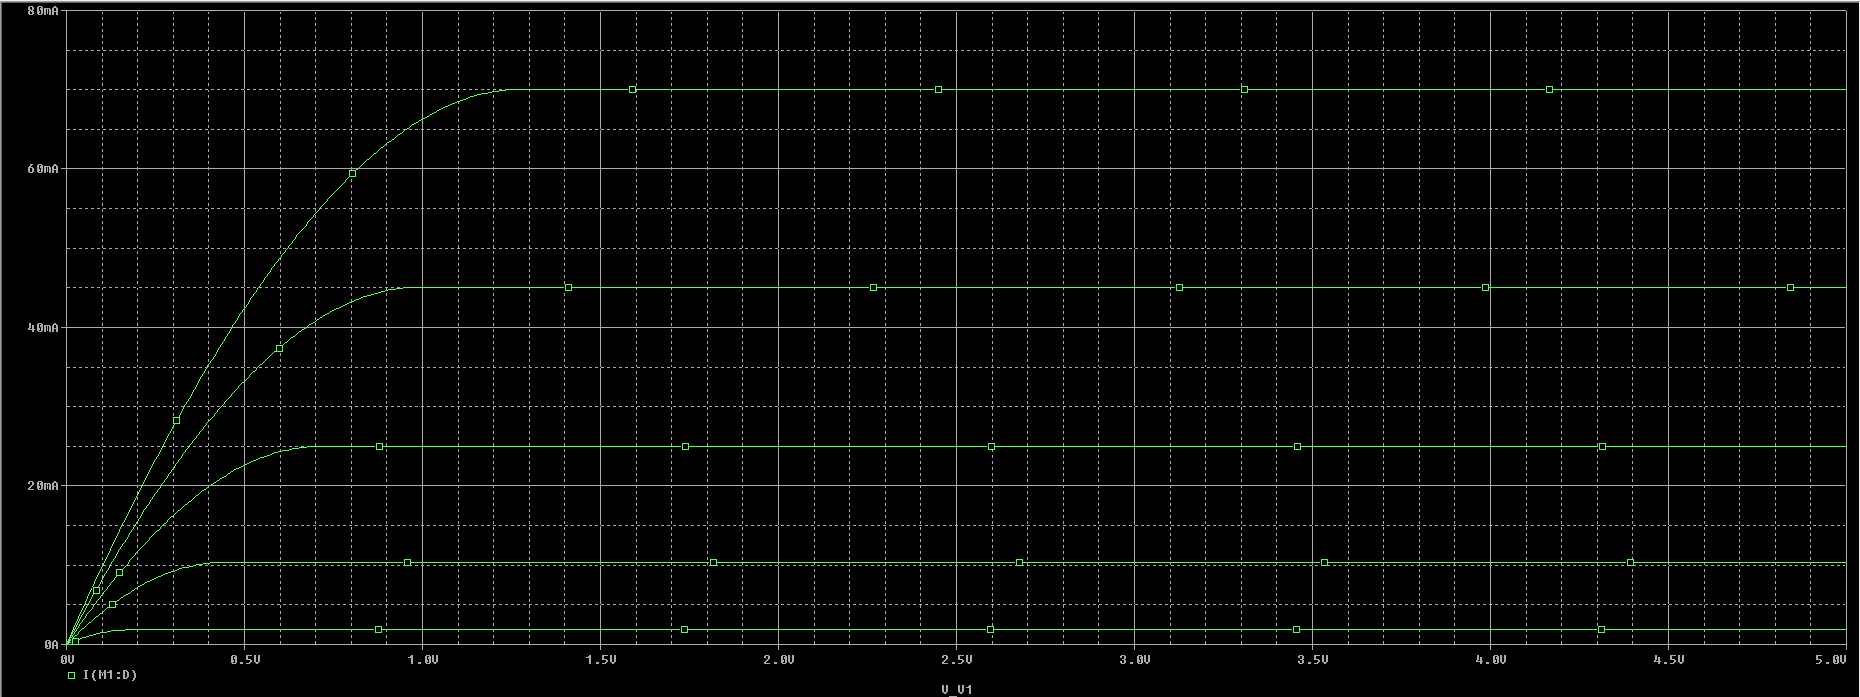
\includegraphics[width=\textwidth]{figures/simulationBase}
\end{center}
\caption{Results from ZETEX BS170/ZTX simulation}
\label{fig:zetexsim}
\end{figure}

\newpage
\subsection{Changing Netlist Parameters}
To model a MOSFET with different parameters you must edit the BS170/ZTX netlist. Click on the BS170/ZTX symbol and select \textbf{Edit $\to$ PSpice Model}. The netlist is under the `Model Text’ heading. The Model Editor is pictured in Figure \ref{fig:netlist}.

\begin{figure}[ht!]
\begin{center}
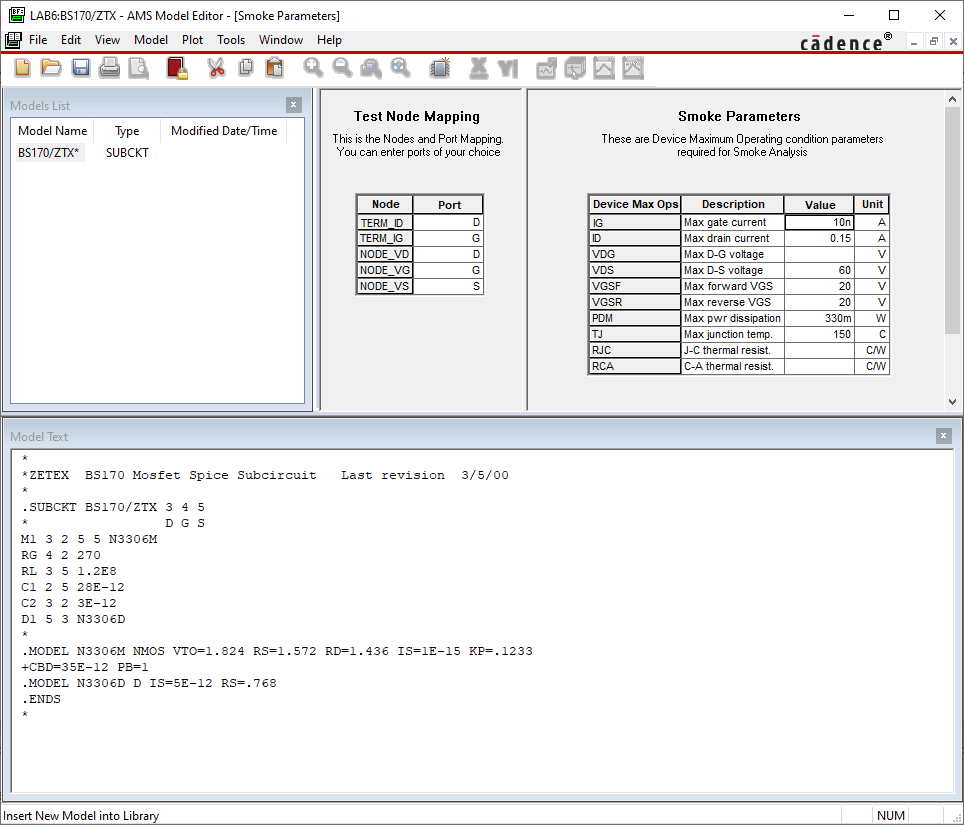
\includegraphics[width=0.65\textwidth]{figures/modelEditor}
\end{center}
\caption{Model editor with original BS170/ZTX netlist}
\label{fig:netlist}
\end{figure}

\subsubsection{Simulating BS170 With Given ZETEX Parameters}
You should have already done this in Section \ref{sim}. Save your results. You will compare these results with the results of simulations with other parameters.

\subsubsection{Simulating Class Average BS170 Parameters}
Replace the parameters in the ``.MODEL\dots'' text with the average extracted parameters. You may need to add a {\tt lambda} parameter. Save the new netlist. Run your simulation and save your results.

\subsubsection{Simulating Manufacturer Specified BS170 Parameters}
Replace the parameters in the ``.MODEL\dots'' text with the parameters found in the Fairchild Semiconductor netlist. Save the new netlist. Run your simulation and save your results.

\textit{Note: The BS170 used in Lab 5 was made by Fairchild Semiconductor. Remember that parameters can vary by manufacturer. The ZETEX and Fairchild Semiconductor parameters may be different.}

Include in your lab the following:
\begin{itemize}
\item A schematic of the circuit used to simulate the MOSFET. Be sure to include all voltage sources in your circuit diagram. This is the PSpice file used to simulate this NMOSFET drain-current characteristics.
\item Three separate plots of the simulation results of $I_D$ vs. $V_{DS}$ for different $V_{GS}$ values for the ZETEX manufacturer, class average measurement, and Fairchild manufacturer.
\item Compare the measured threshold voltage, transconductance, and channel-length modulation parameters for the ZETEX manufacturer, class average measurement, and Fairchild manufacturer. Comment on how these three parameters affect the PSpice simulated output plots.
\end{itemize}

\section{Extension}
\begin{itemize}
\item Which parameter in PSpice most affects the MOSFET I-V curve?  Discuss what changing these parameters would mean in a circuit in real life?  You may use the simple Lab 6 MOSFET circuit when considering the device output
\item What semiconductor effects are at play for each parameter in the MOSFET?  Be sure to relate the parameter with the effect it has on MOSFET performance.
\item Discuss what make one device parameter ``better'' than another.  Be sure to define what you consider, ``better.''  Based on your definition of ``better,'' which MOSFET from lab---the manufacturer's, actual lab averaged, or PSpice---is better by your definition?
\item Explore in depth another question that piqued your interest as you completed this laboratory.
\end{itemize}

%____________________________________________________________________________
%
%	Grading Rubric
%____________________________________________________________________________
\newpage
\def\arraystretch{1.2}
\phantomsection
\addcontentsline{toc}{section}{Grading Rubric}
\markboth{Grading Rubric}{Grading Rubric}
\hspace{0pt}
\vfill % used to center table vertically on page
\begin{table}[ht!]
\caption{ECE 230L Laboratory 6 Grading Rubric}
\centering
\begin{tabular}{l|c} \hline
Criteria & Points Possible \\ \hline \hline
\textbf{Circuit Schematic used to simulate MOSFET}	& \textbf{10} \\ \hline
\textbf{Verification of ZETEX BS170 Plots}			& \textbf{8} \\ \hline
\textbf{ZETEX Manufacturer specified BS170 parameter simulation}		& \textbf{15} \\
Plot of $I_{DS}$ vs $V_{DS}(V_{GS})$ 				& 15 \\ \hline
\textbf{Class average BS170 parameter simulation}	& \textbf{20} \\
Average Calculation									& 5 \\ 
Plot of $I_{DS}$ vs $V_{DS}(V_{GS})$ 				& 15 \\ \hline
\textbf{Fairchild Manufacturer specified BS170 parameter simulation}		& \textbf{15} \\
Plot of $I_{DS}$ vs $V_{DS}(V_{GS})$ 				& 15 \\ \hline
\textbf{Compare values of $V_{TH}, K_p$, and $\lambda$ for all three simulations} & \textbf{15} \\ \hline
\textbf{Comment on the effects of $V_{TH}, K_p$, and $\lambda$ on the graphs} & \textbf{10} \\ \hline
{\bf Extension} 									& {\bf 7} \\ \hline \hline
{\bf Total}											& {\bf 100} \\ \hline
\end{tabular}
\end{table}
\vfill % used to center table vertically on page
\end{document}
